\chapter{高层设计}
通过全局,虽然我们对该系统采用的是微服务架构,但是纵向来说,对于某个具体的模块,我们依然采用传统的MVC模式,即区分视图层、业务层和持久层。
视图层负责和前端进行数据交互,业务层负责业务逻辑处理,持久层负责和数据库进行数据交互,三层各司其职,实现系统的可控、可扩展。本章针对需求规格说明书提出
的需求进行提炼,给出本系统的层次结构,包括包图、部署图等设计。

\section{模块图}
系统中我们分为了许多Modules,主要为4个模块,Common、Service、GateWay、NacosCore,其作用分别是通用工具模块,微服务业务模块,网管模块和服务注册中心模块,
下面图~\ref{fig:Modules}~给出了系统的总体模块图。
\begin{figure}[htbp]
    \centering
    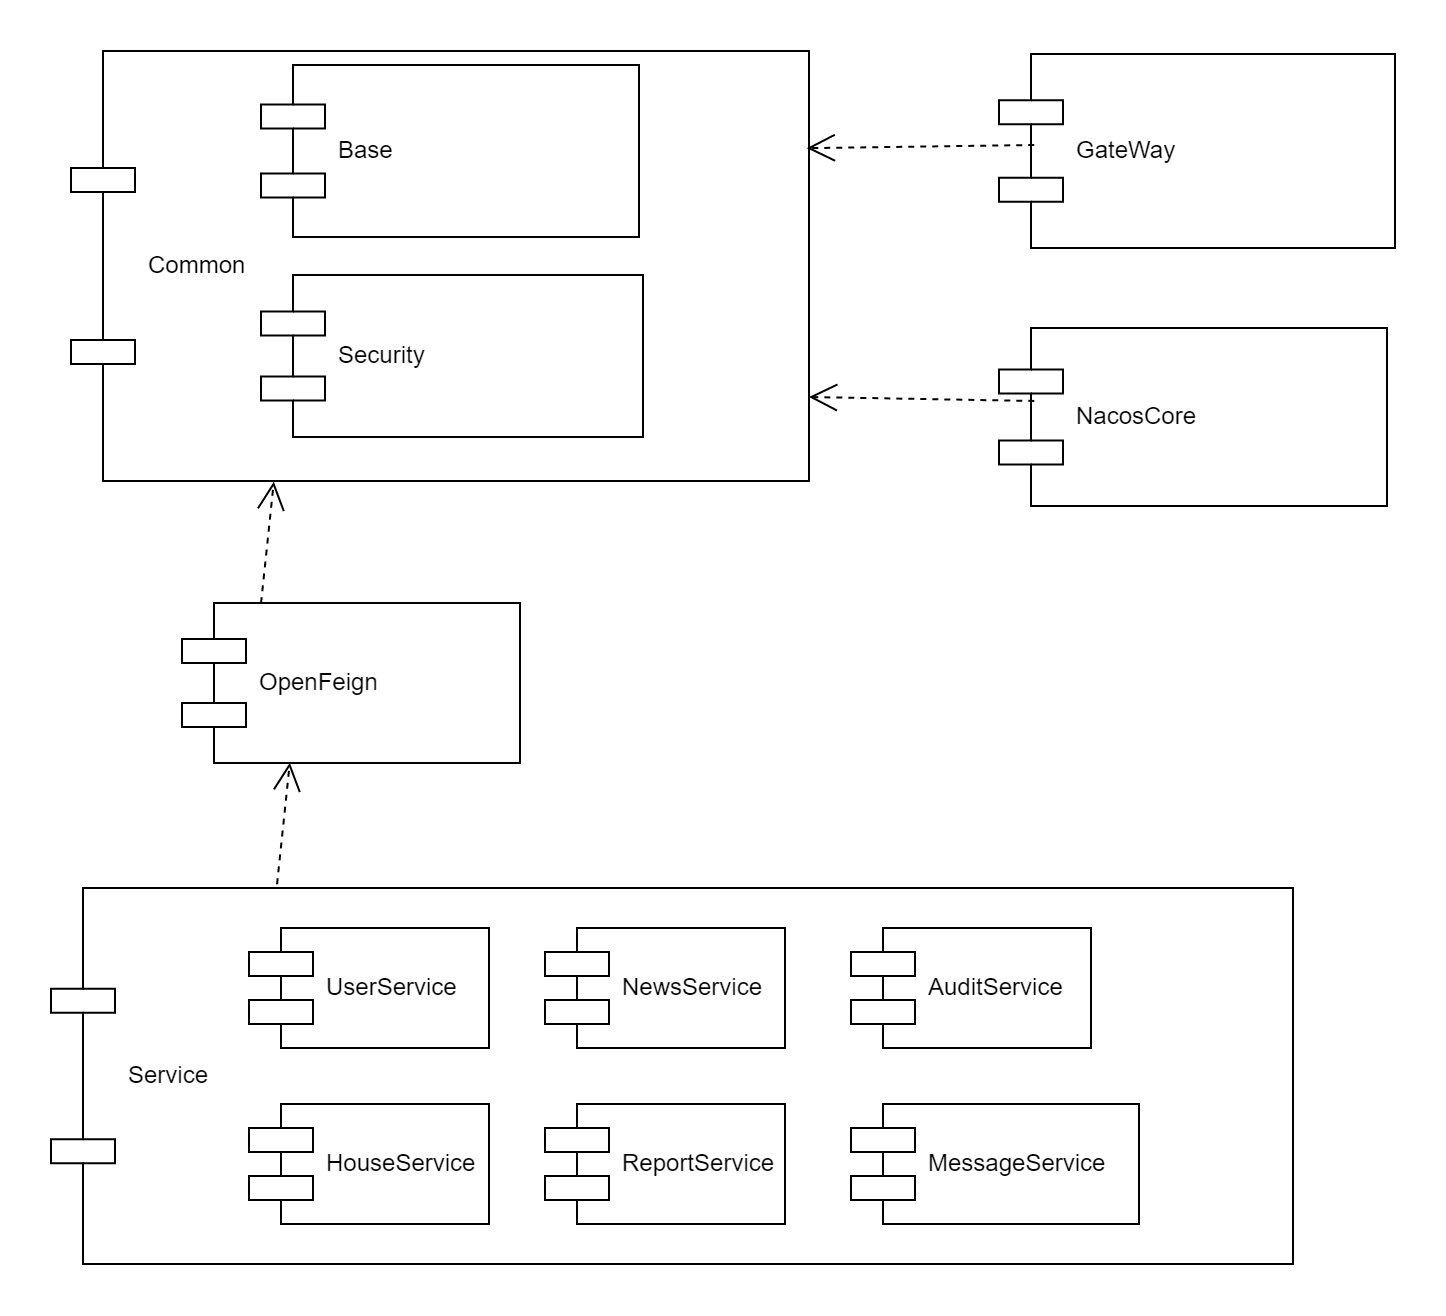
\includegraphics[width=\textwidth]{ch3/Modules.jpg}
    \caption{模块图}\label{fig:Modules}
    \vspace{\baselineskip} % 表示图与正文空一行
\end{figure}

其中四个模块还含有不同的子模块,我们对于四个模块的作用及其子模块做一个大致说明。
\begin{itemize}
    \item Common通用工具模块,将其他模块通用的功能抽象成一个独立的模块,便于调用。
    \begin{itemize}
        \item Base模块,包含了一些基本配置,比如Redis缓存的配置,返回类的配置等等。
        \item Security模块,整合了SpringSecurity框架,用于对用户进行认证授权。
    \end{itemize}
    \item Service微服务业务模块,即负责系统实际业务的模块,将所有业务统一到一个父类模块下,便于统一配置。
    \begin{itemize}
        \item UserService模块,负责处理用户信息的模块,包括用户登录、用户注册、管理获取用户列表等。
        \item HouseService模块,负责处理房源帖子的信息,包括发帖、改贴、帖子列表等。
        \item ReportService模块,负责举报信息,包括发起举报,审核举报等。
        \item NewsService模块,负责管理新闻信息,包括编辑新闻,获取新闻列表等。
        \item AuditService模块,负责管理审核信息,包括举报审核、新闻审核等。
        \item MessageService模块,负责处理系统的消息和通知,用于管理员给用户群发通知等。
    \end{itemize}
    \item GateWay网管模块,负责分发路由,将请求转发到对应的微服务上,同时也负责初步校验JWT,检验用户身份。
    \item NacosCore微服务注册中心模块,负责管理系统中的各项微服务,包括服务注册、服务发现、流量监控等。
\end{itemize}

\section{包图}
接下来我们来设计各个模块中的包结构,不同功能的模块有着不同的包结构。大体来说,业务模块主要以MVC模式为主,即不同的层次对应不同的包,而配置相关的模块则
会根据配置类别进行不同的分包。

\subsection{Common通用工具模块}
Common模块中包含两个子模块,为Base模块和Security模块。
\subsubsection{Base}
Base中主要包含两个包,分别是Config和Util,分别负责一些全局参数的配置。Config中包含了Redis、RestTemplate、Constant(全局常量)的配置。Util中包含了ResponseUtil(统一返回设置)、Result(统一返回类)等全局统一用的配置。
Base模块的总体包图如图~\ref{fig:Base}~所示。
\begin{figure}[htbp]
    \centering
    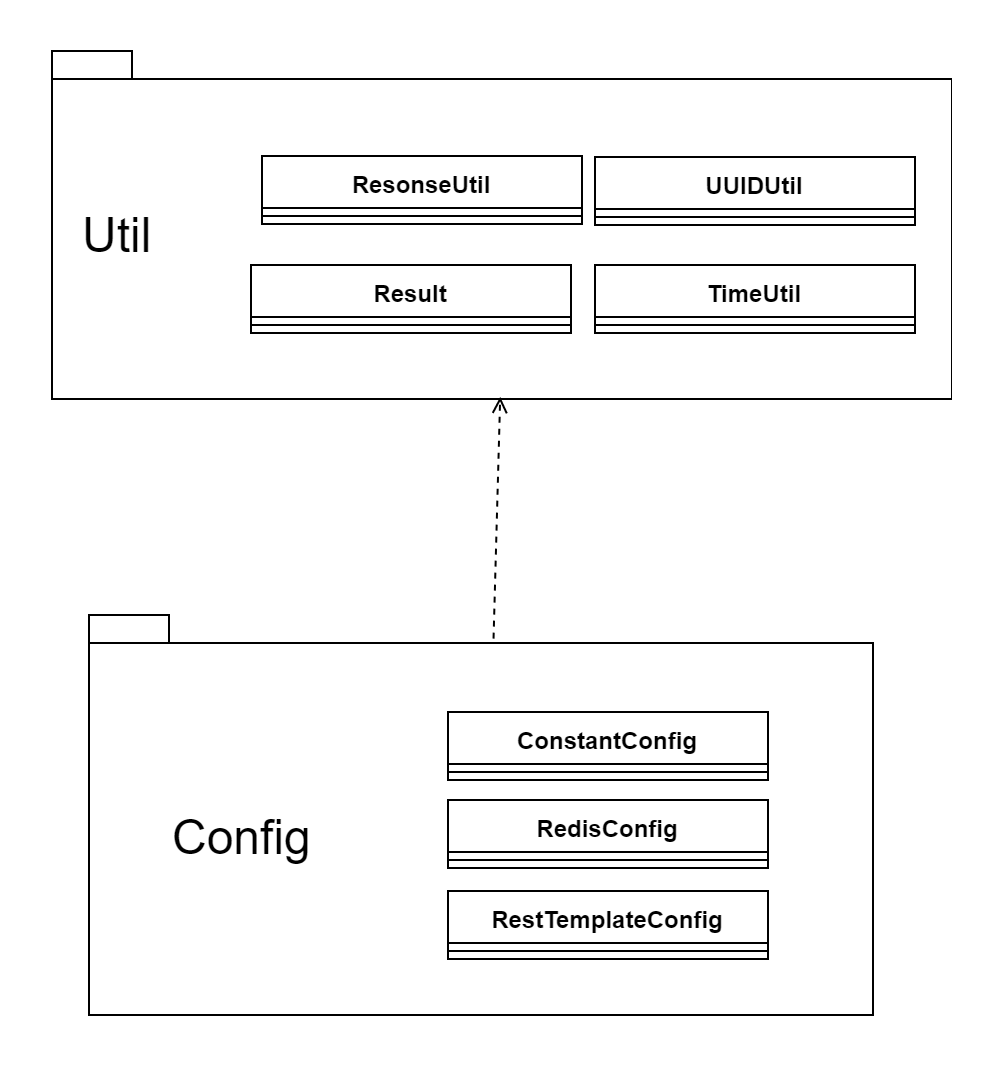
\includegraphics[width=0.6\textwidth]{ch3/Base.jpg}
    \caption{Base模块包图}\label{fig:Base}
    \vspace{\baselineskip} % 表示图与正文空一行
\end{figure}

\subsubsection{Security}
Security中主要包含4个包,为Config、Filter、Entity、Security。其中,Config为安全框架的具体配置,Filter中自定了一些过滤器,Entity中定义了一些实体类,Security中定义了具体的认证授权操作类。
Security模块的总体包图如图~\ref{fig:Security}~所示。
\begin{figure}[htbp]
    \centering
    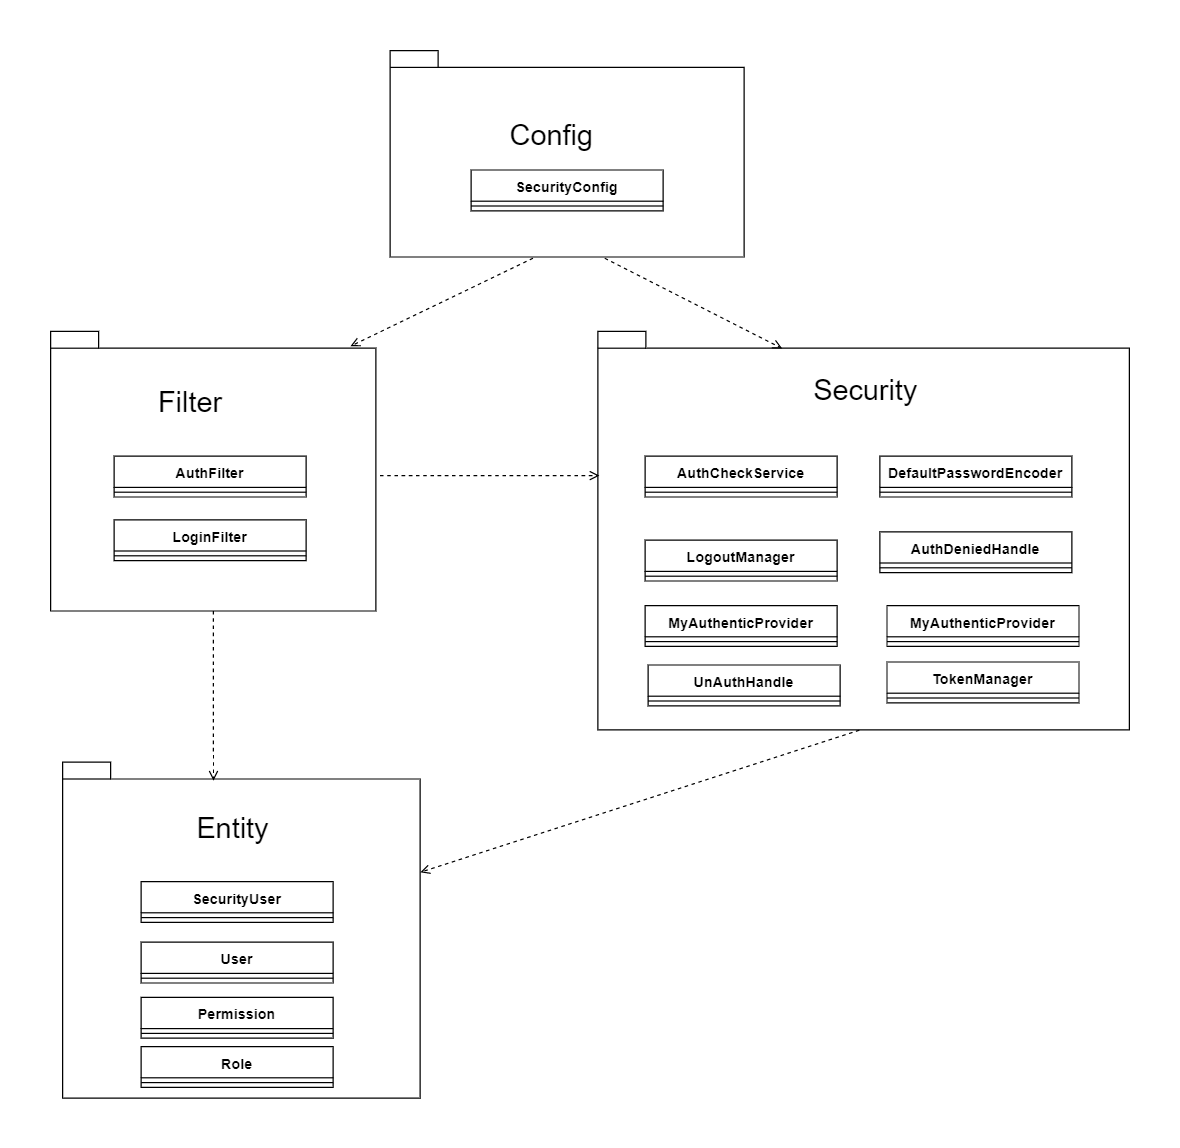
\includegraphics[width=\textwidth]{ch3/Security.jpg}
    \caption{Security模块包图}\label{fig:Security}
    \vspace{\baselineskip} % 表示图与正文空一行
\end{figure}

\subsection{Service微服务业务模块}
Service模块包含6个子模块,为UserService模块、HouseService模块、NewsService模块、ReportService模块、AuditService模块、MessageService模块。

\subsubsection{UserService}
UserService模块主要包含6个包,主要是MVC模式下的几个包,包括Controller、Service、Impl、Dao、Entity、Vo。前5个包的功能在前文均有描述,而Vo包的主要
功能是统一该模块的前端传来的数据模型,比如UserForm,以及后端返回给前端的数据模型,比如UserVo。
UserService模块的总体包图如图~\ref{fig:UserService}~所示。
\begin{figure}[htbp]
    \centering
    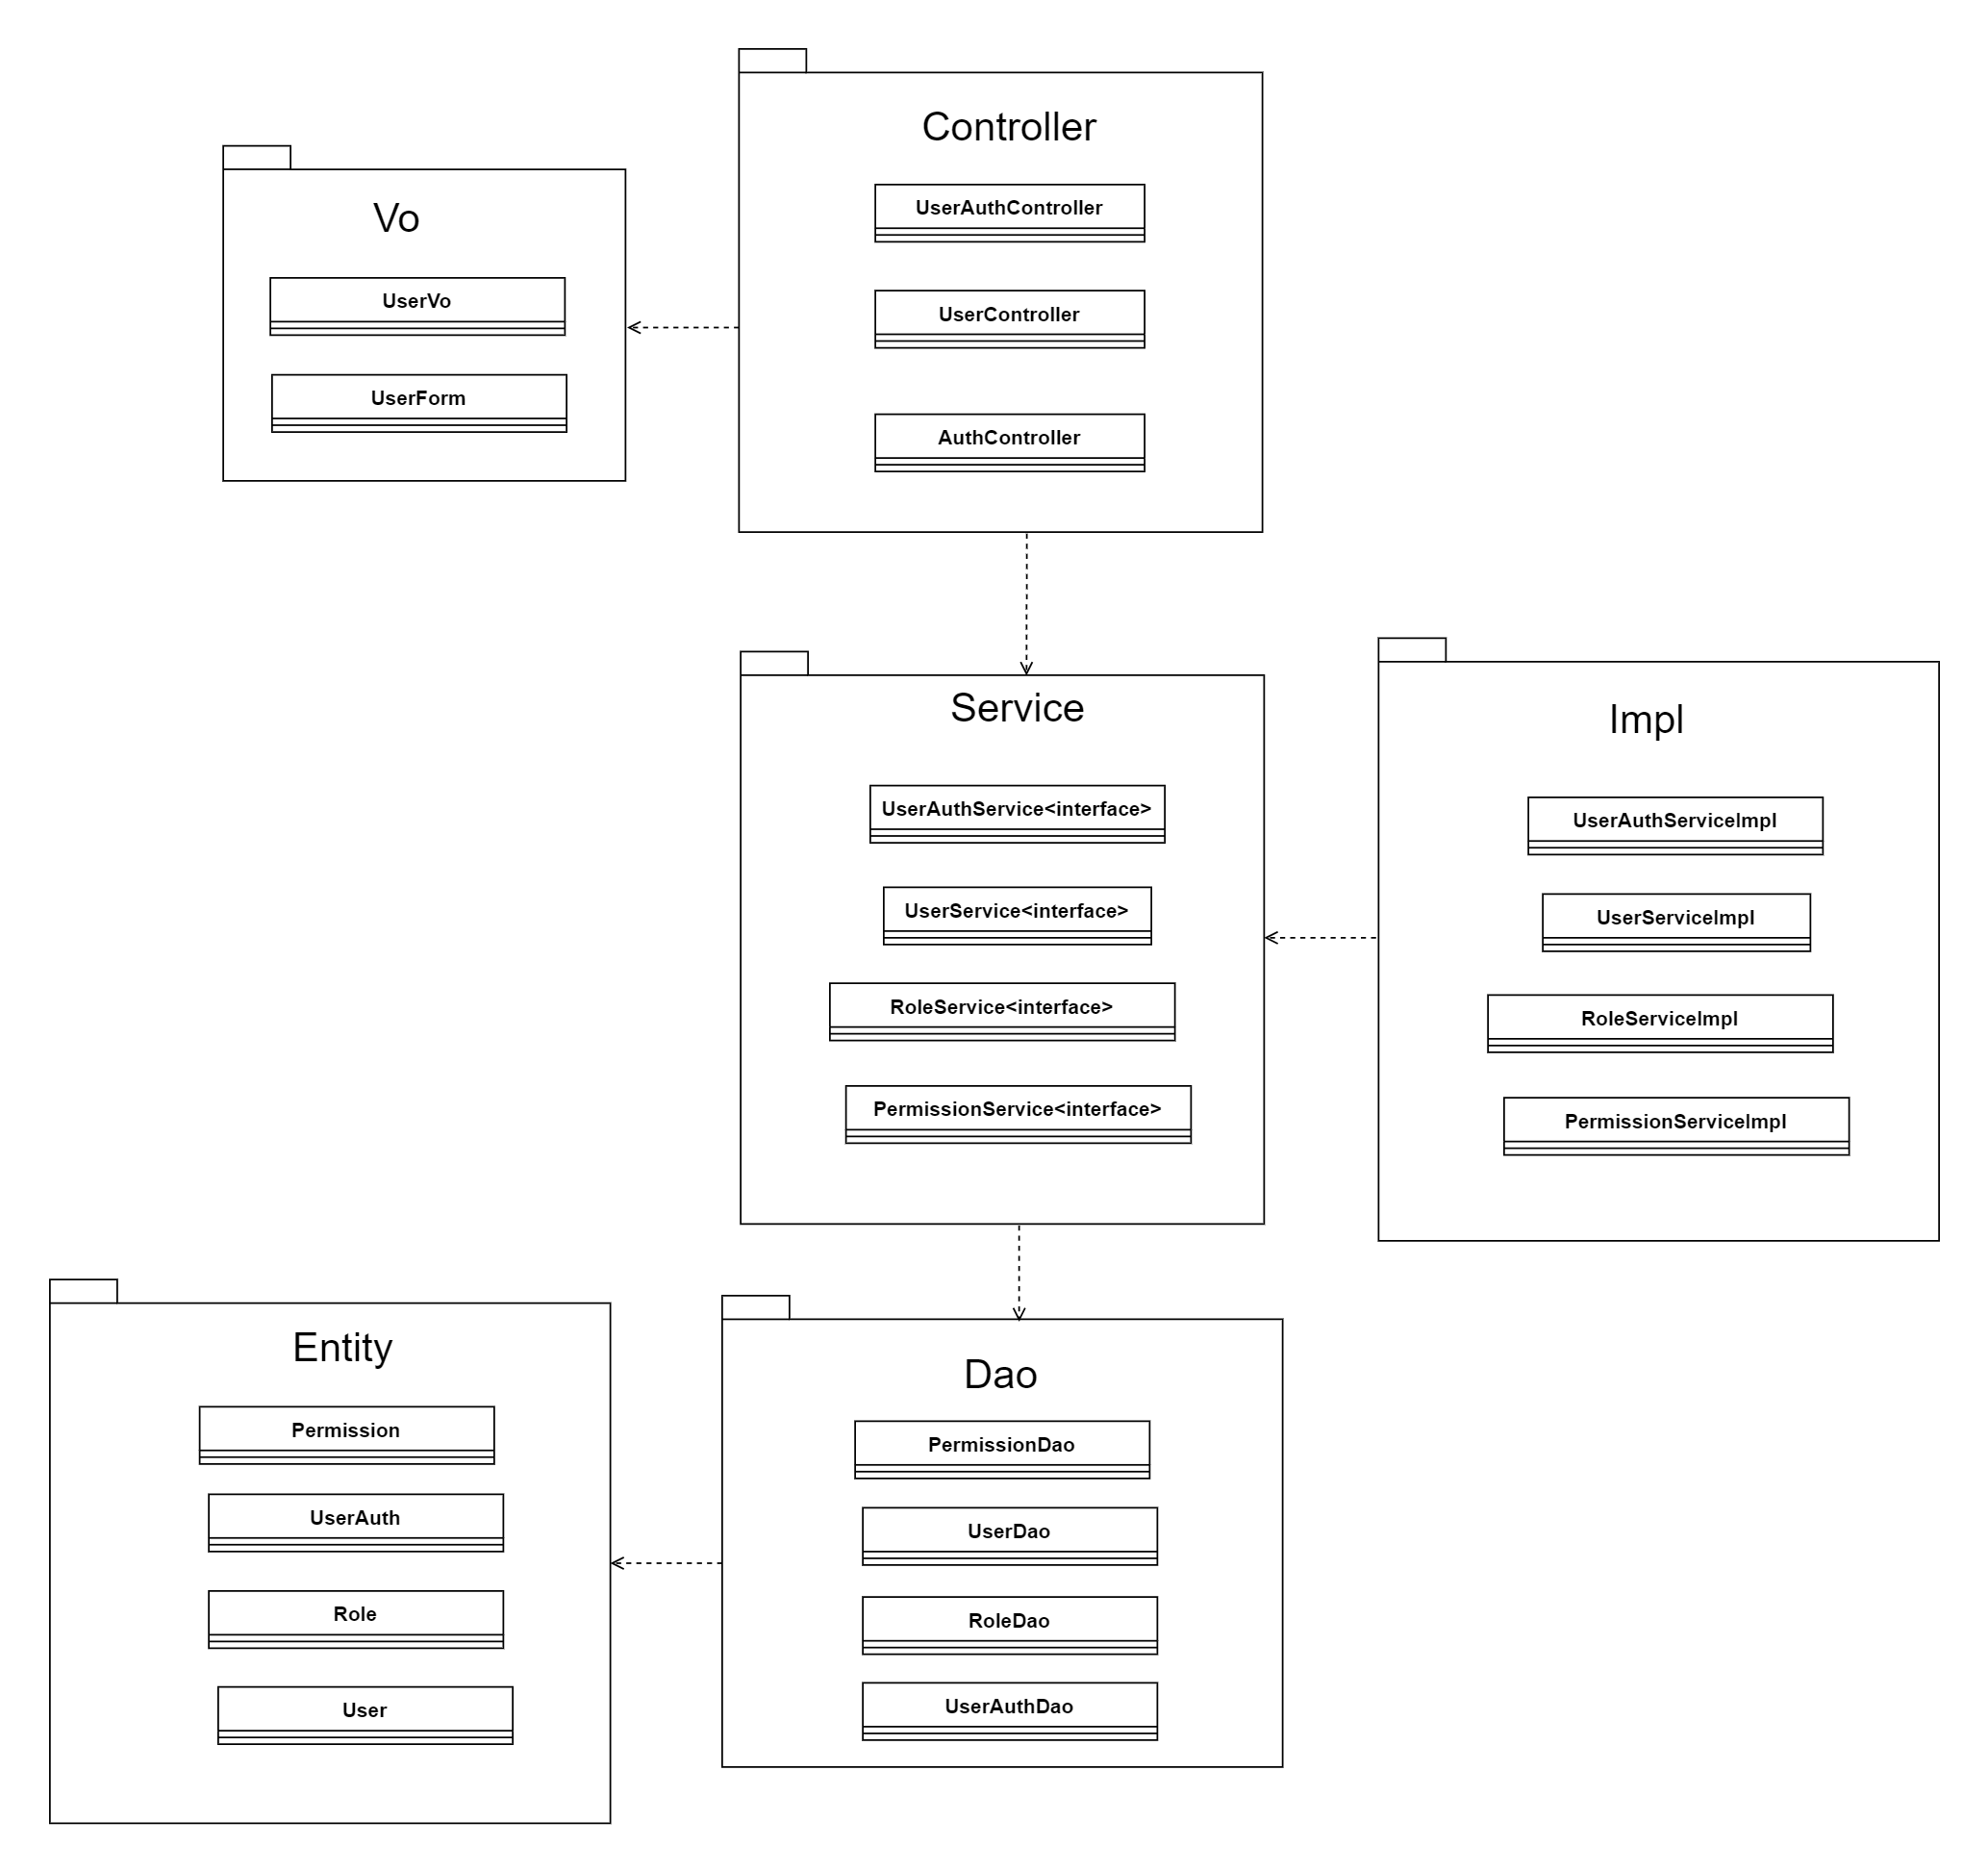
\includegraphics[width=\textwidth]{ch3/UserService.png}
    \caption{UserService模块包图}\label{fig:UserService}
    \vspace{\baselineskip} % 表示图与正文空一行
\end{figure}


\subsubsection{HouseService}
HouseService模块和上文一样,也包含6个包。总体包图如图所示。
\begin{figure}[htbp]
    \centering
    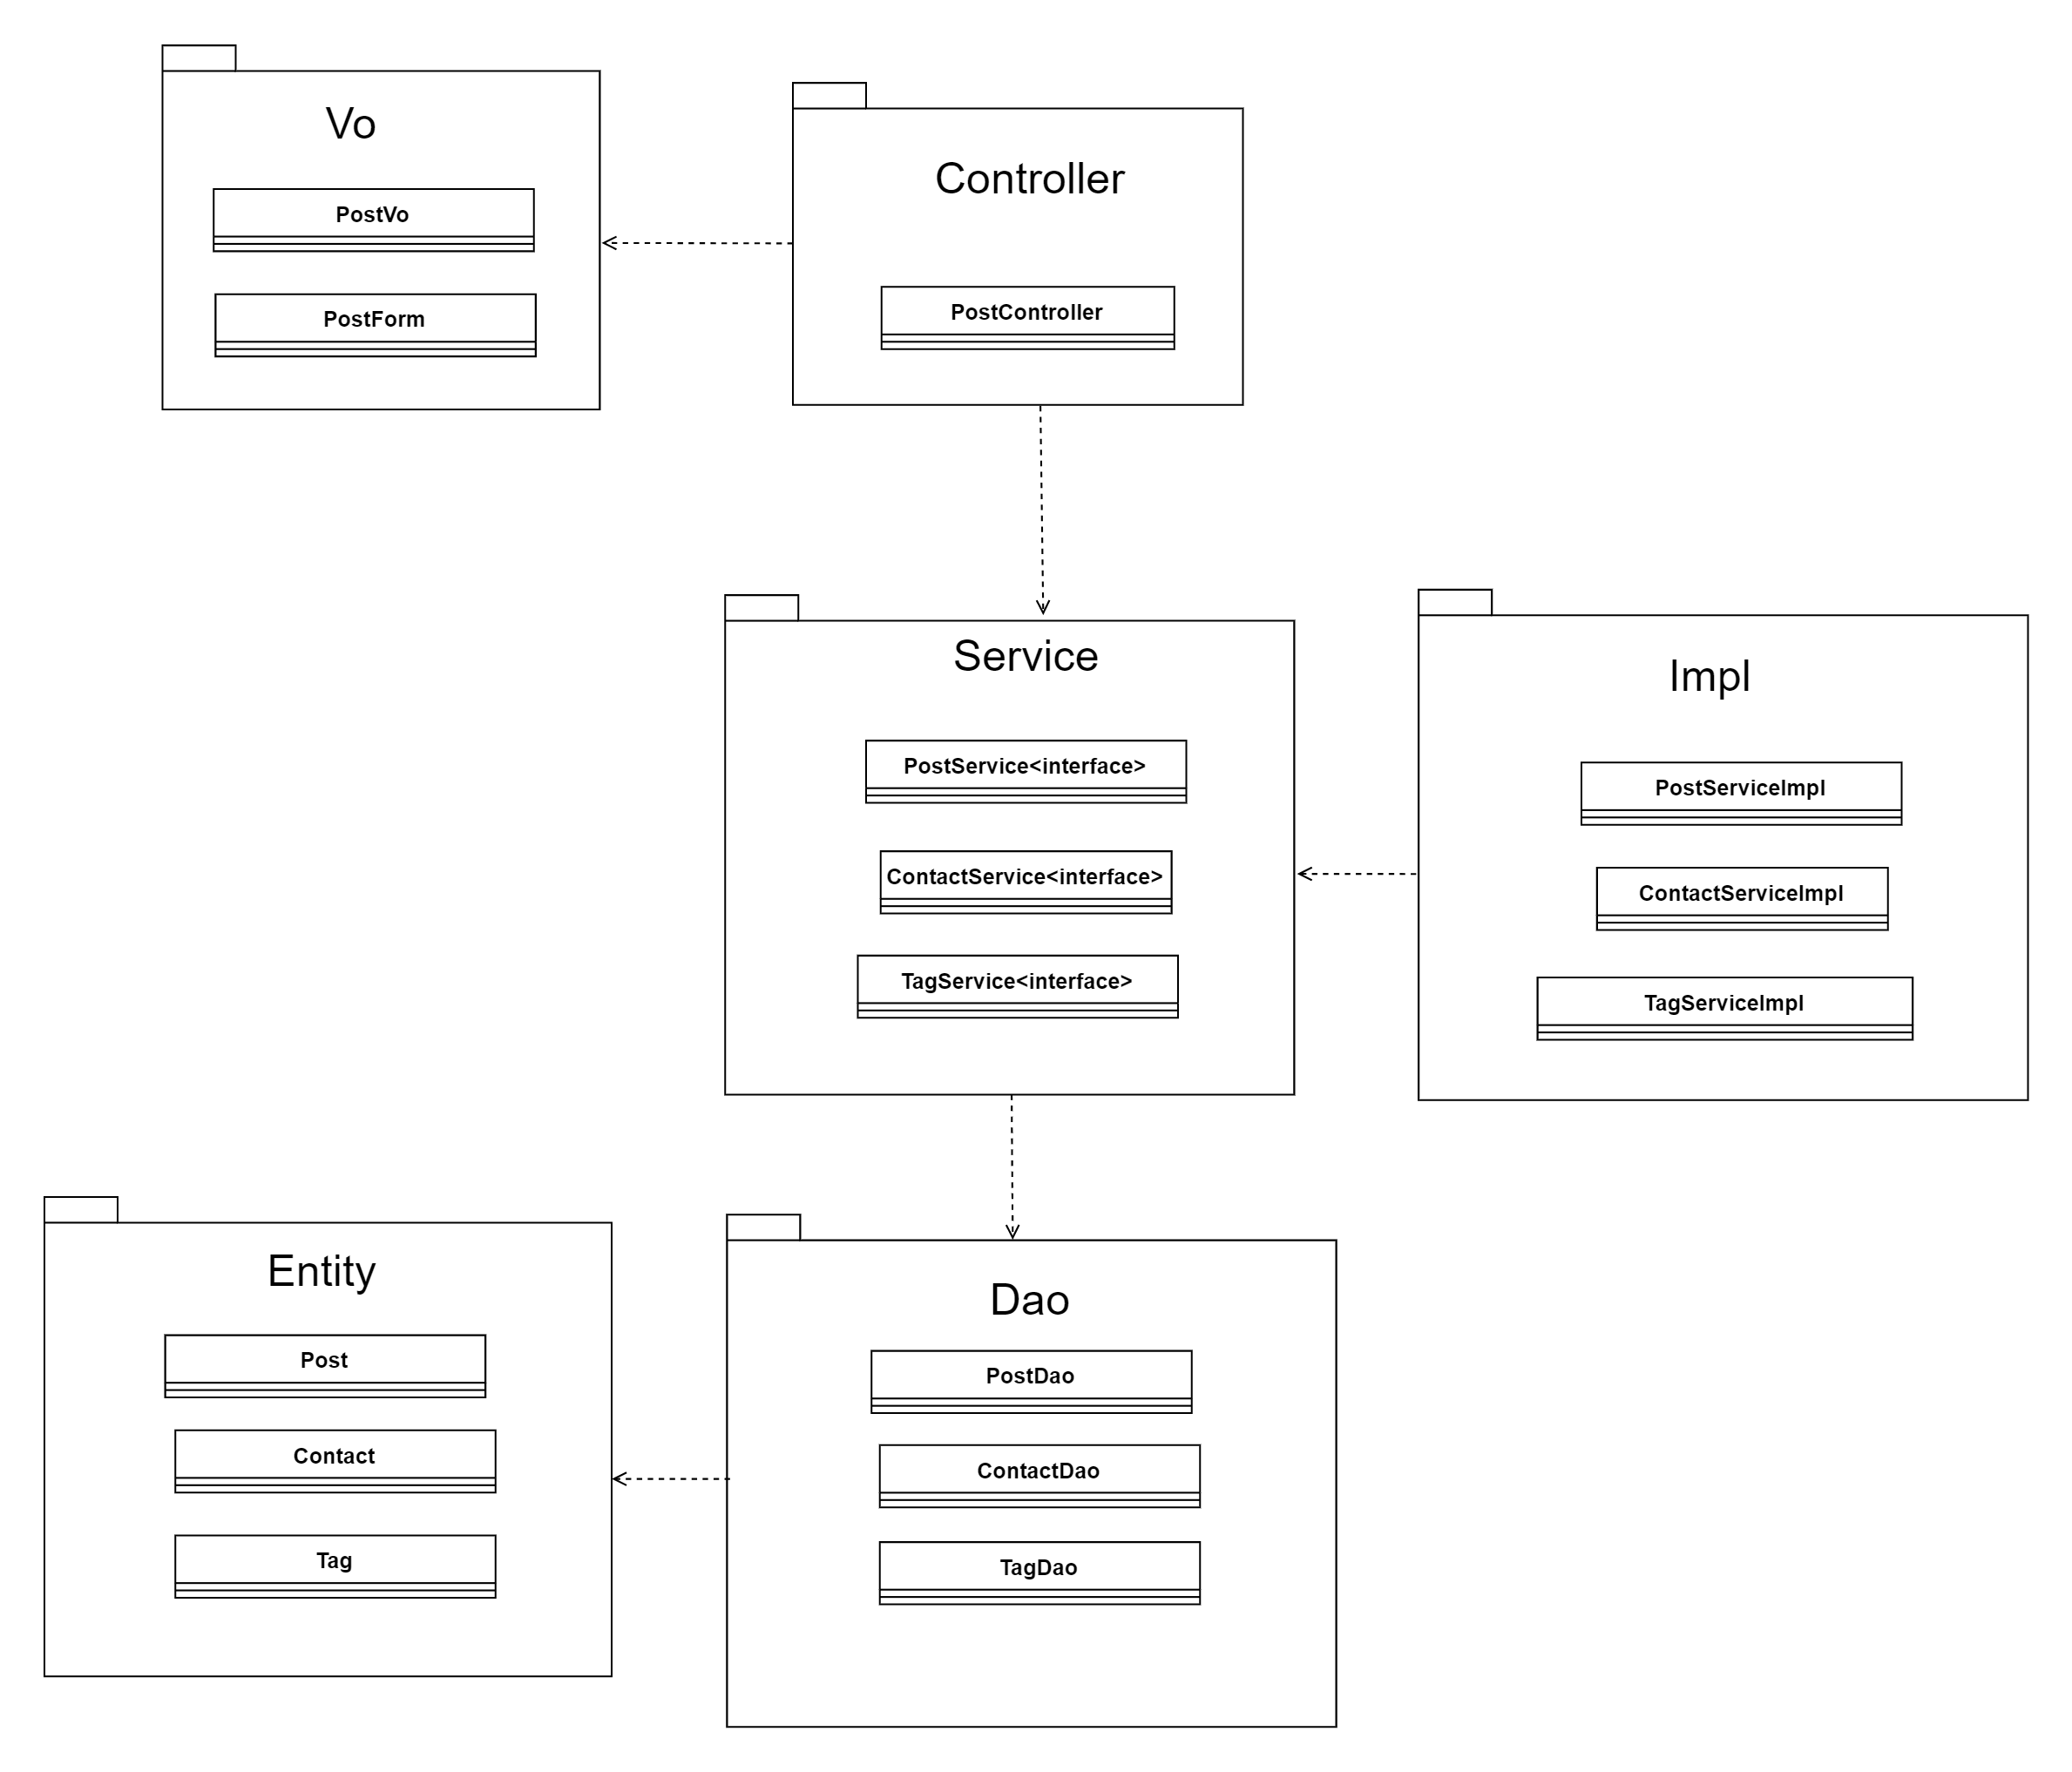
\includegraphics[width=\textwidth]{ch3/HouseService.jpg}
    \caption{HouseService模块包图}\label{fig:HouseService}
    \vspace{\baselineskip} % 表示图与正文空一行
\end{figure}

\subsubsection{NewsService}
包含6个包,总体包图如图~\ref{fig:NewsService}~所示。
\begin{figure}[htbp]
    \centering
    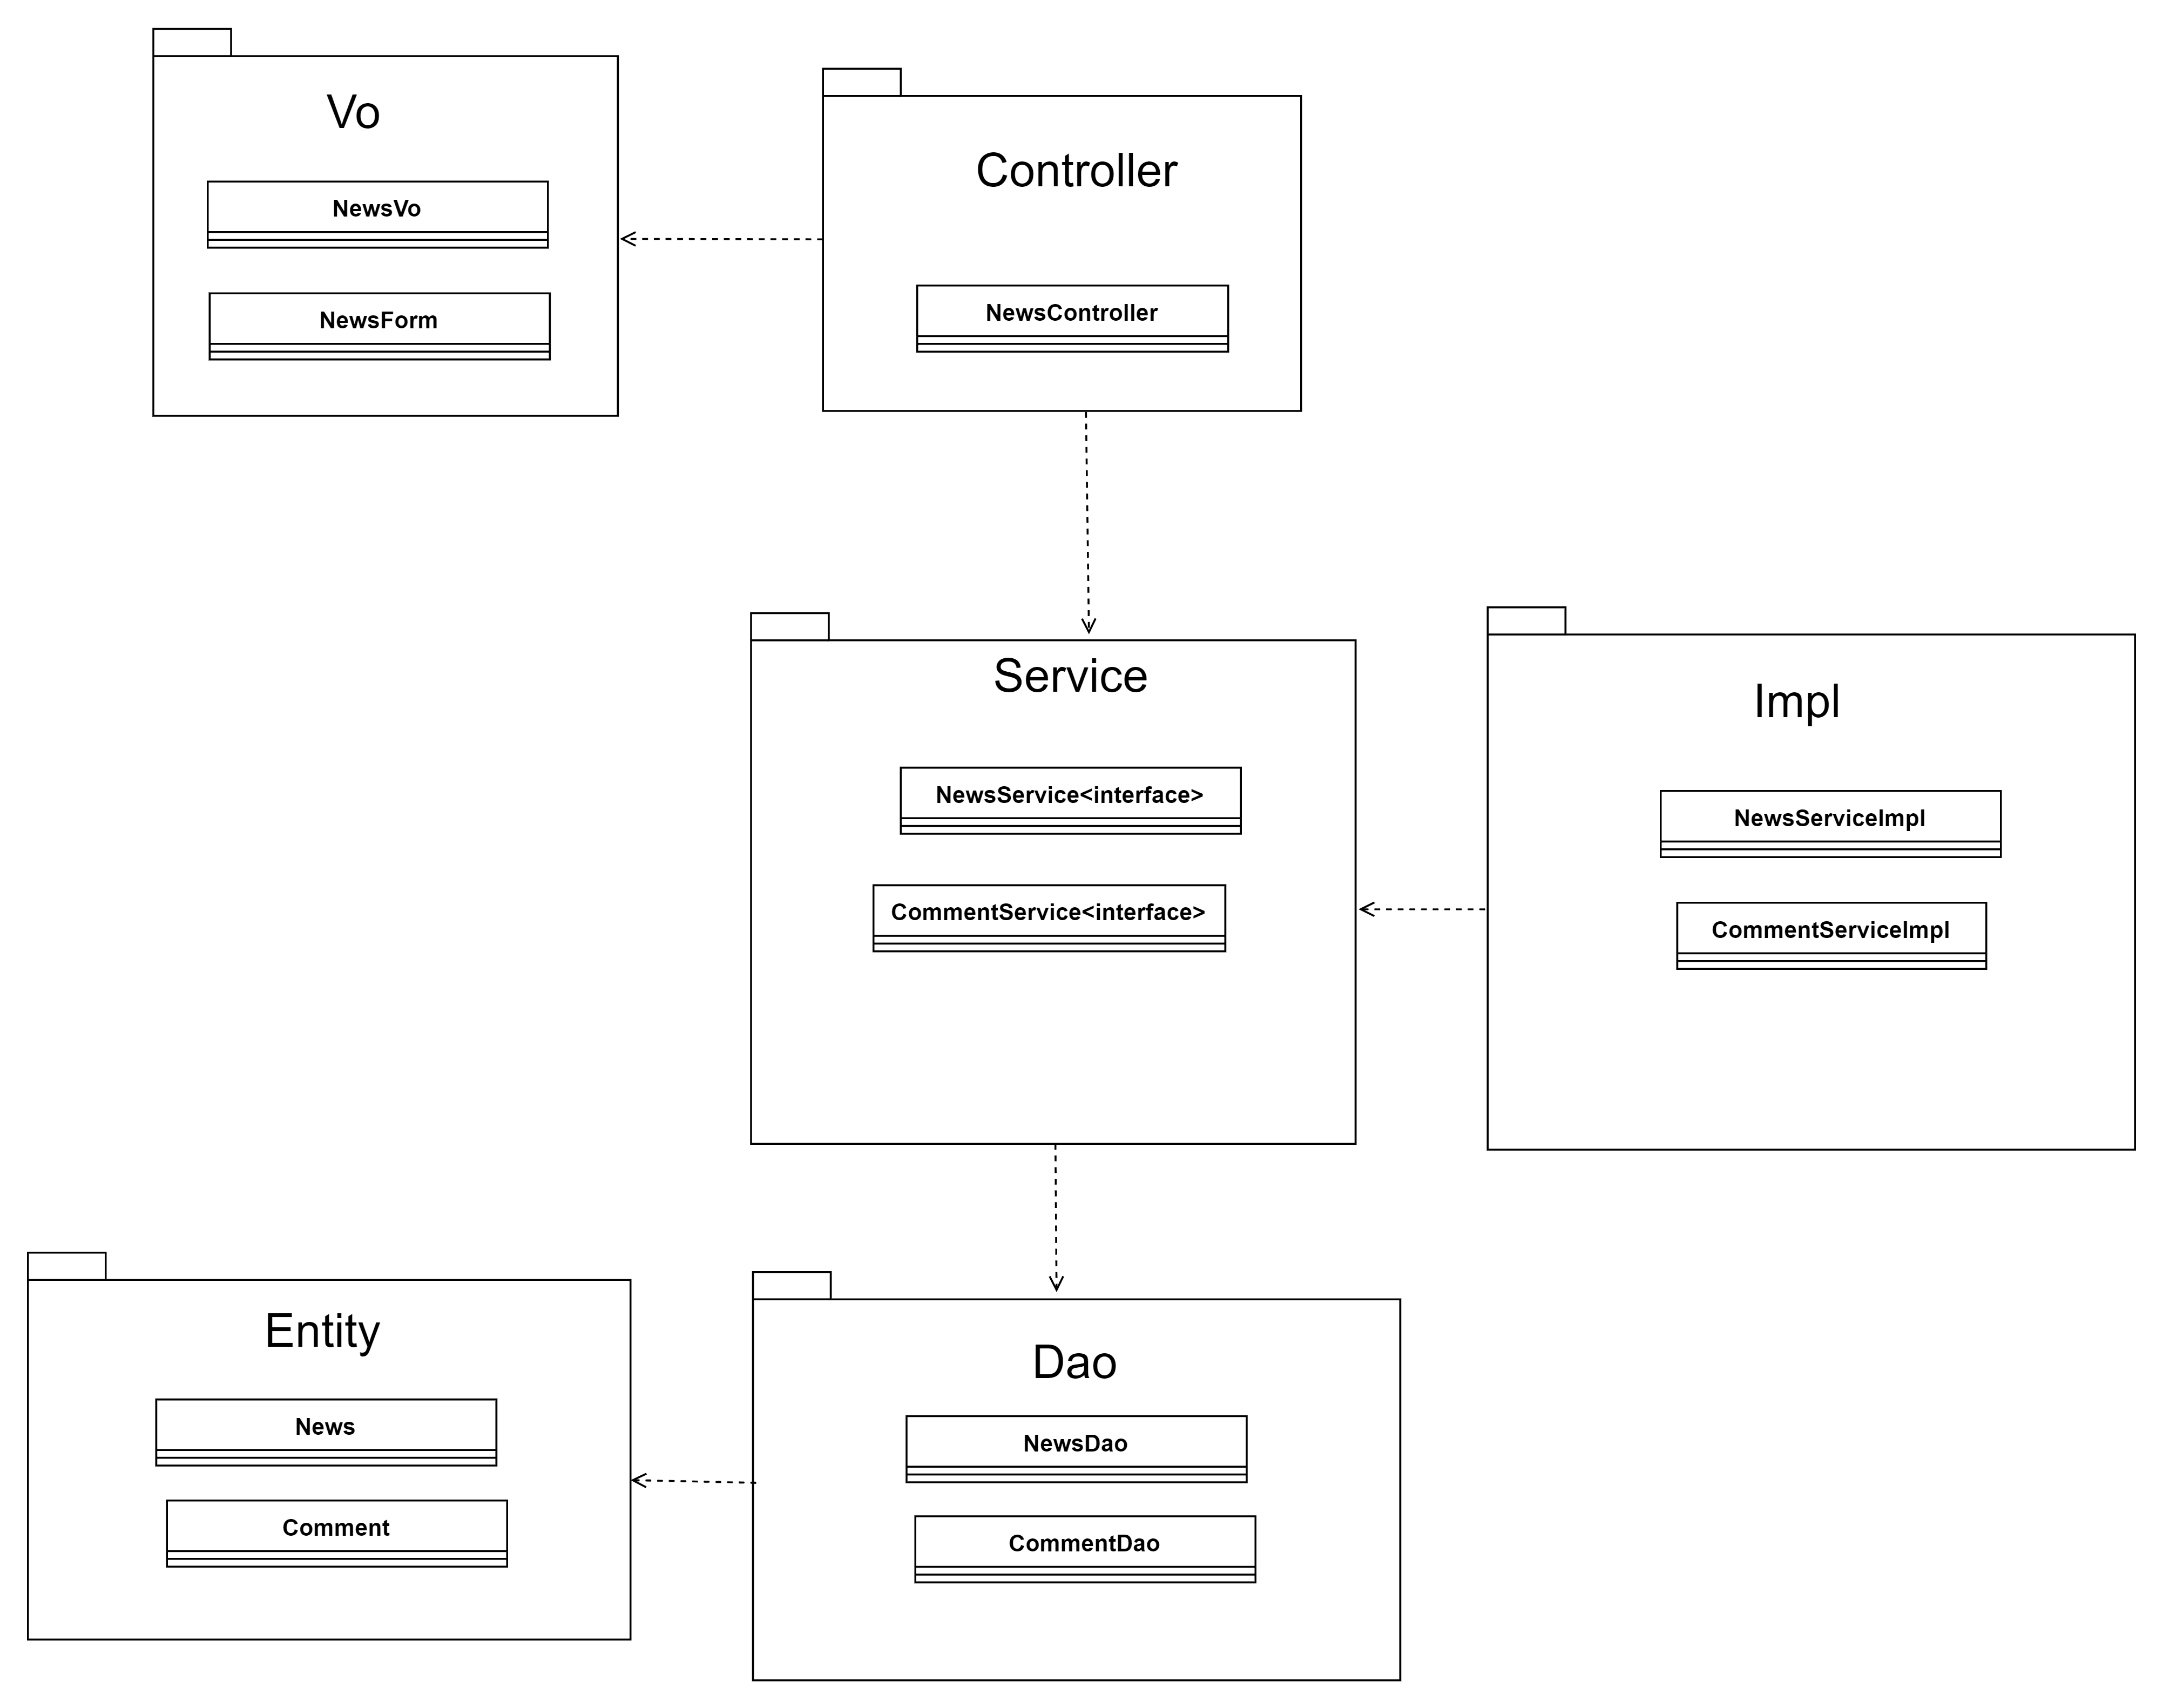
\includegraphics[width=\textwidth]{ch3/NewsService.jpg}
    \caption{NewsService模块包图}\label{fig:NewsService}
    \vspace{\baselineskip} % 表示图与正文空一行
\end{figure}

\subsubsection{ReportService}
包含6个包,总体包图如图~\ref{fig:ReportService}~所示。
\begin{figure}[htbp]
    \centering
    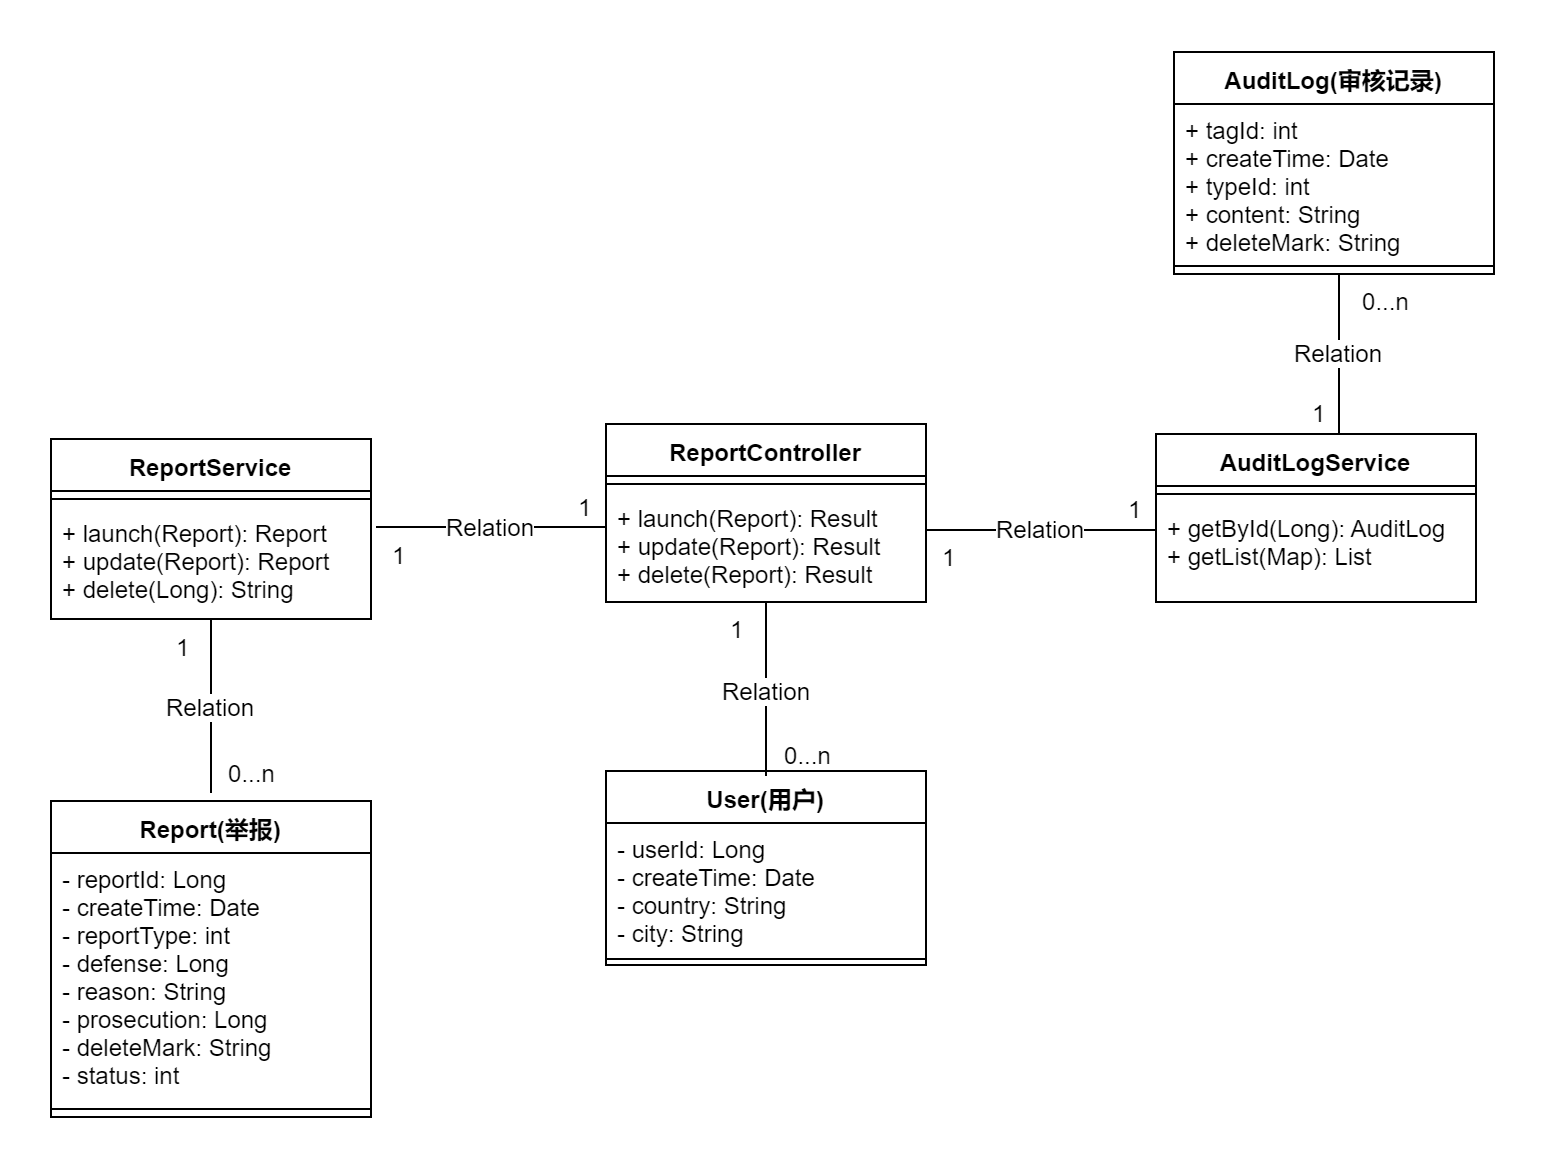
\includegraphics[width=\textwidth]{ch3/ReportService.jpg}
    \caption{ReportService模块包图}\label{fig:ReportService}
    \vspace{\baselineskip} % 表示图与正文空一行
\end{figure}

\subsubsection{AuditService}
包含6个包,总体包图如图~\ref{fig:AuditReport}~所示。
\begin{figure}[htbp]
    \centering
    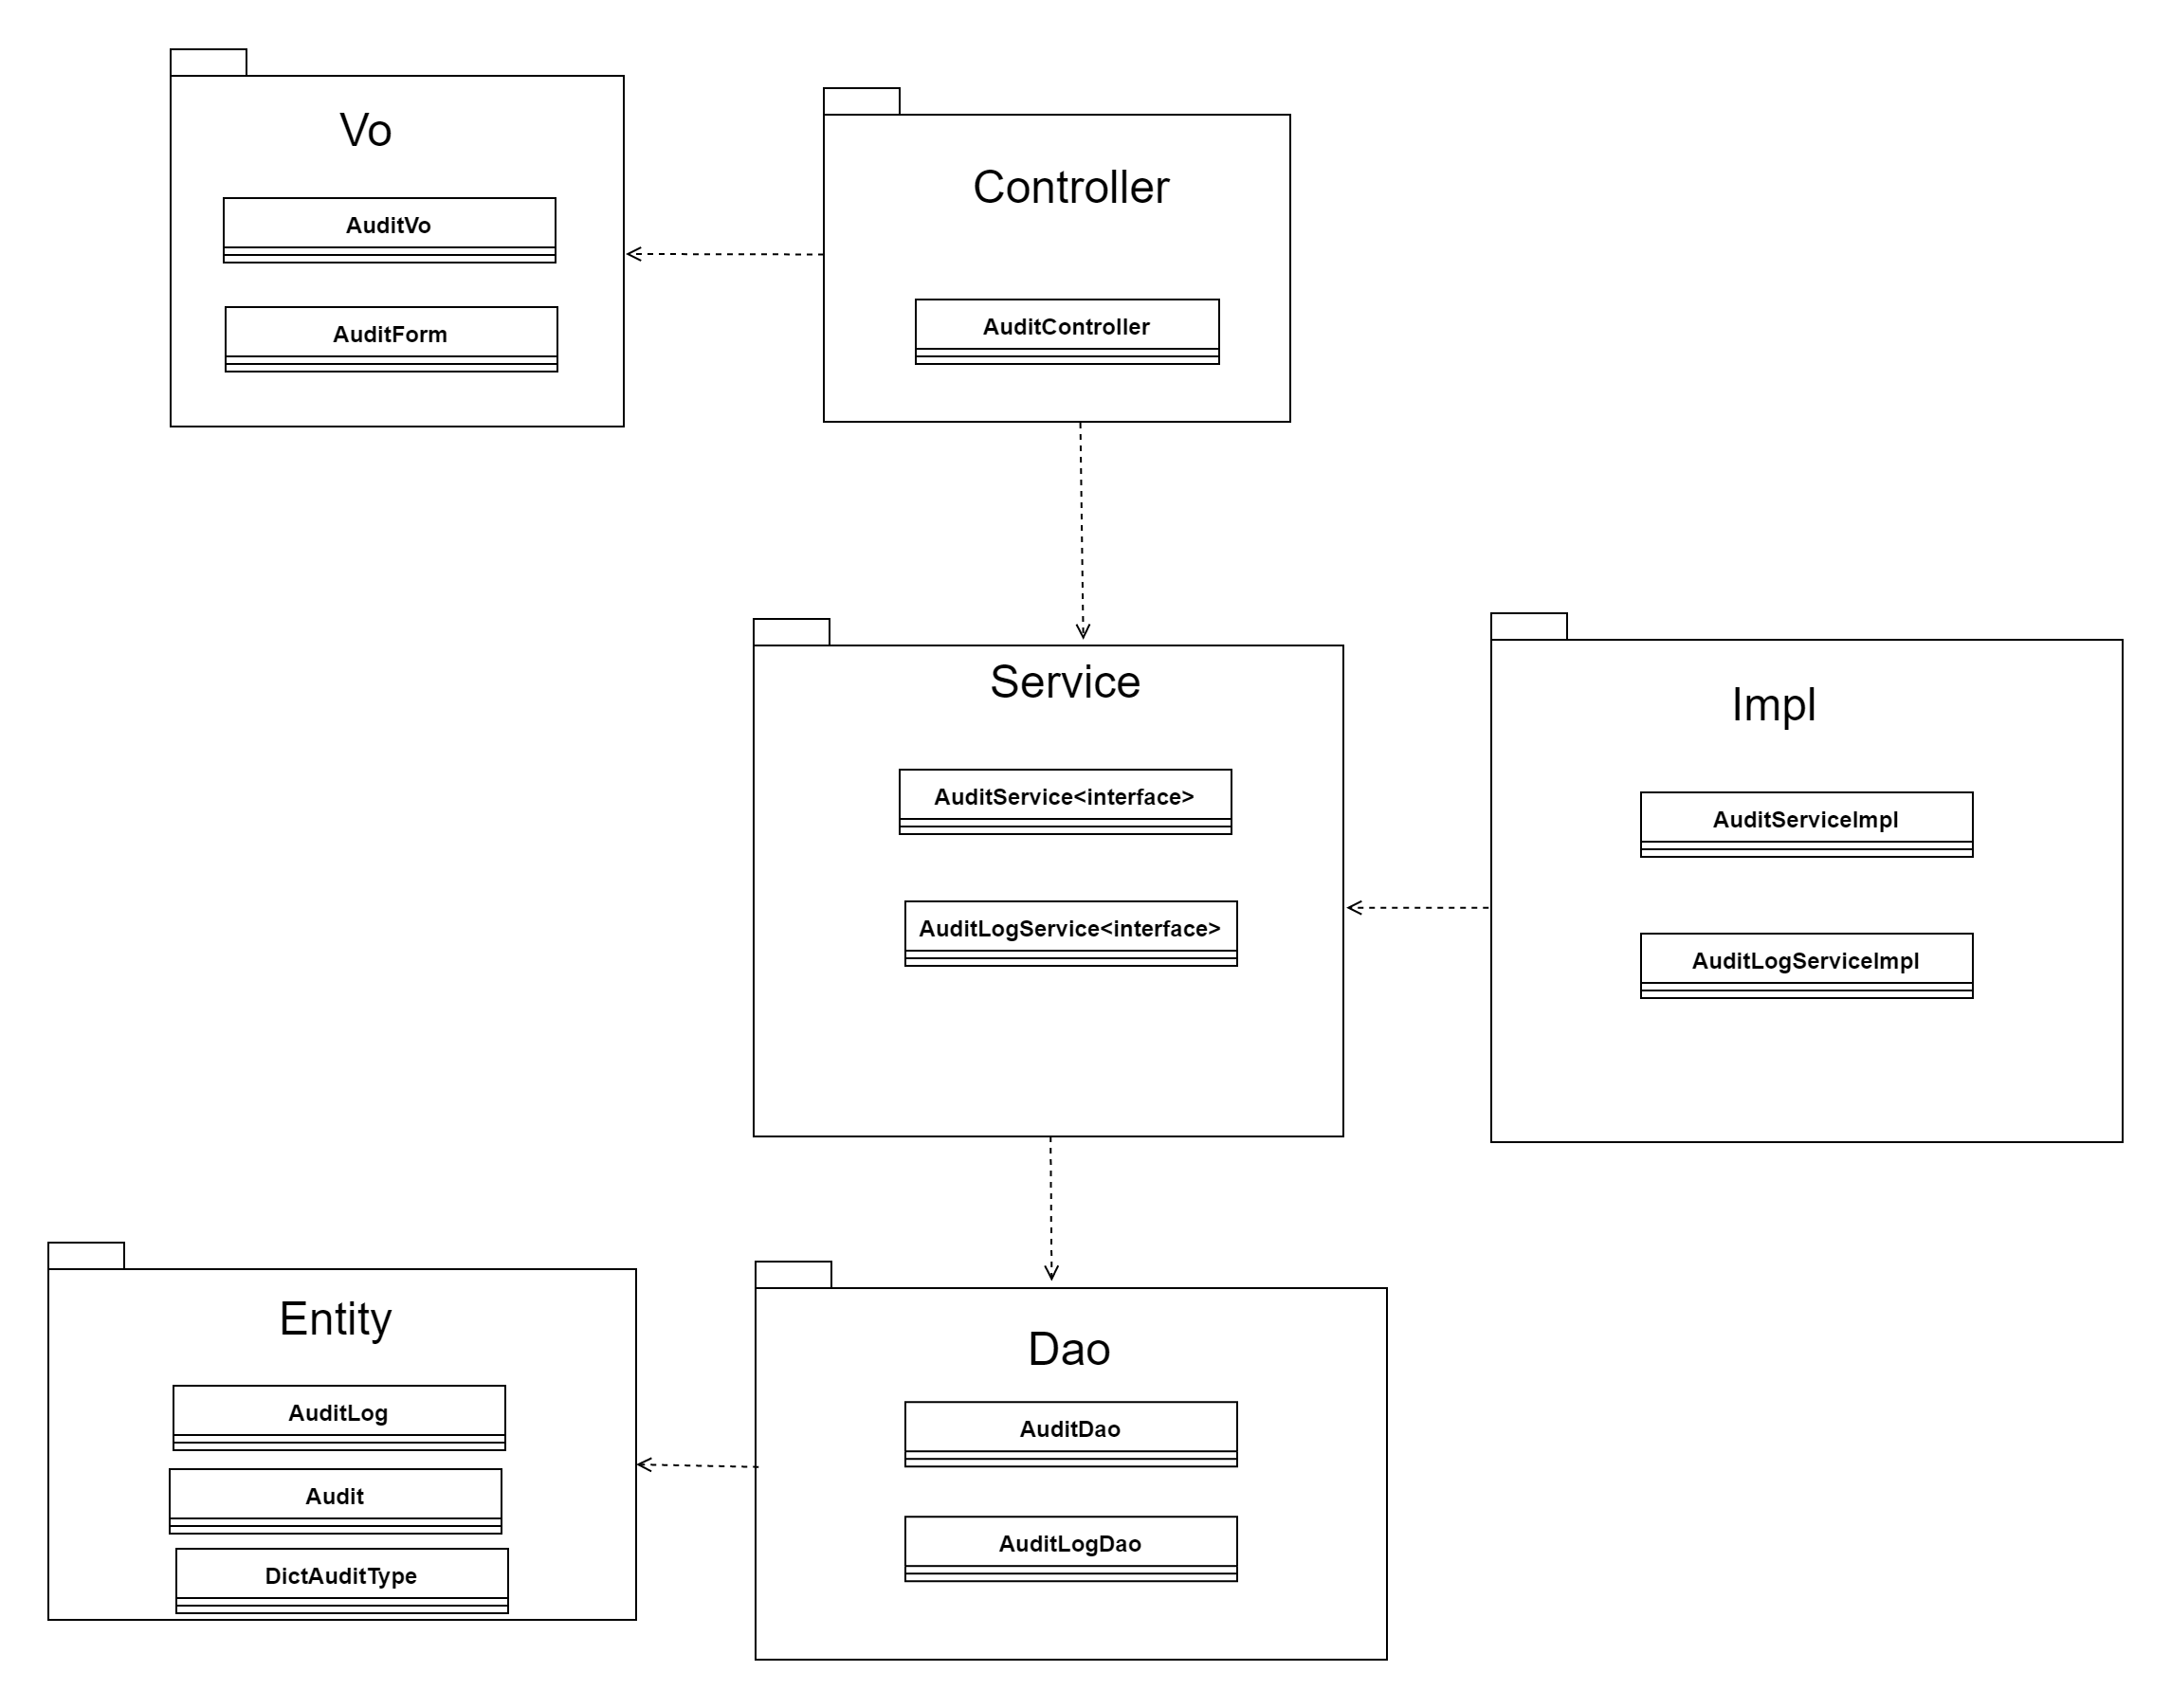
\includegraphics[width=\textwidth]{ch3/AuditService.jpg}
    \caption{AuditService模块包图}\label{fig:AuditService}
    \vspace{\baselineskip} % 表示图与正文空一行
\end{figure}

\subsubsection{MessageService}
包含6个包,总体包图如图~\ref{fig:AuditReport}~所示。
\begin{figure}[htbp]
    \centering
    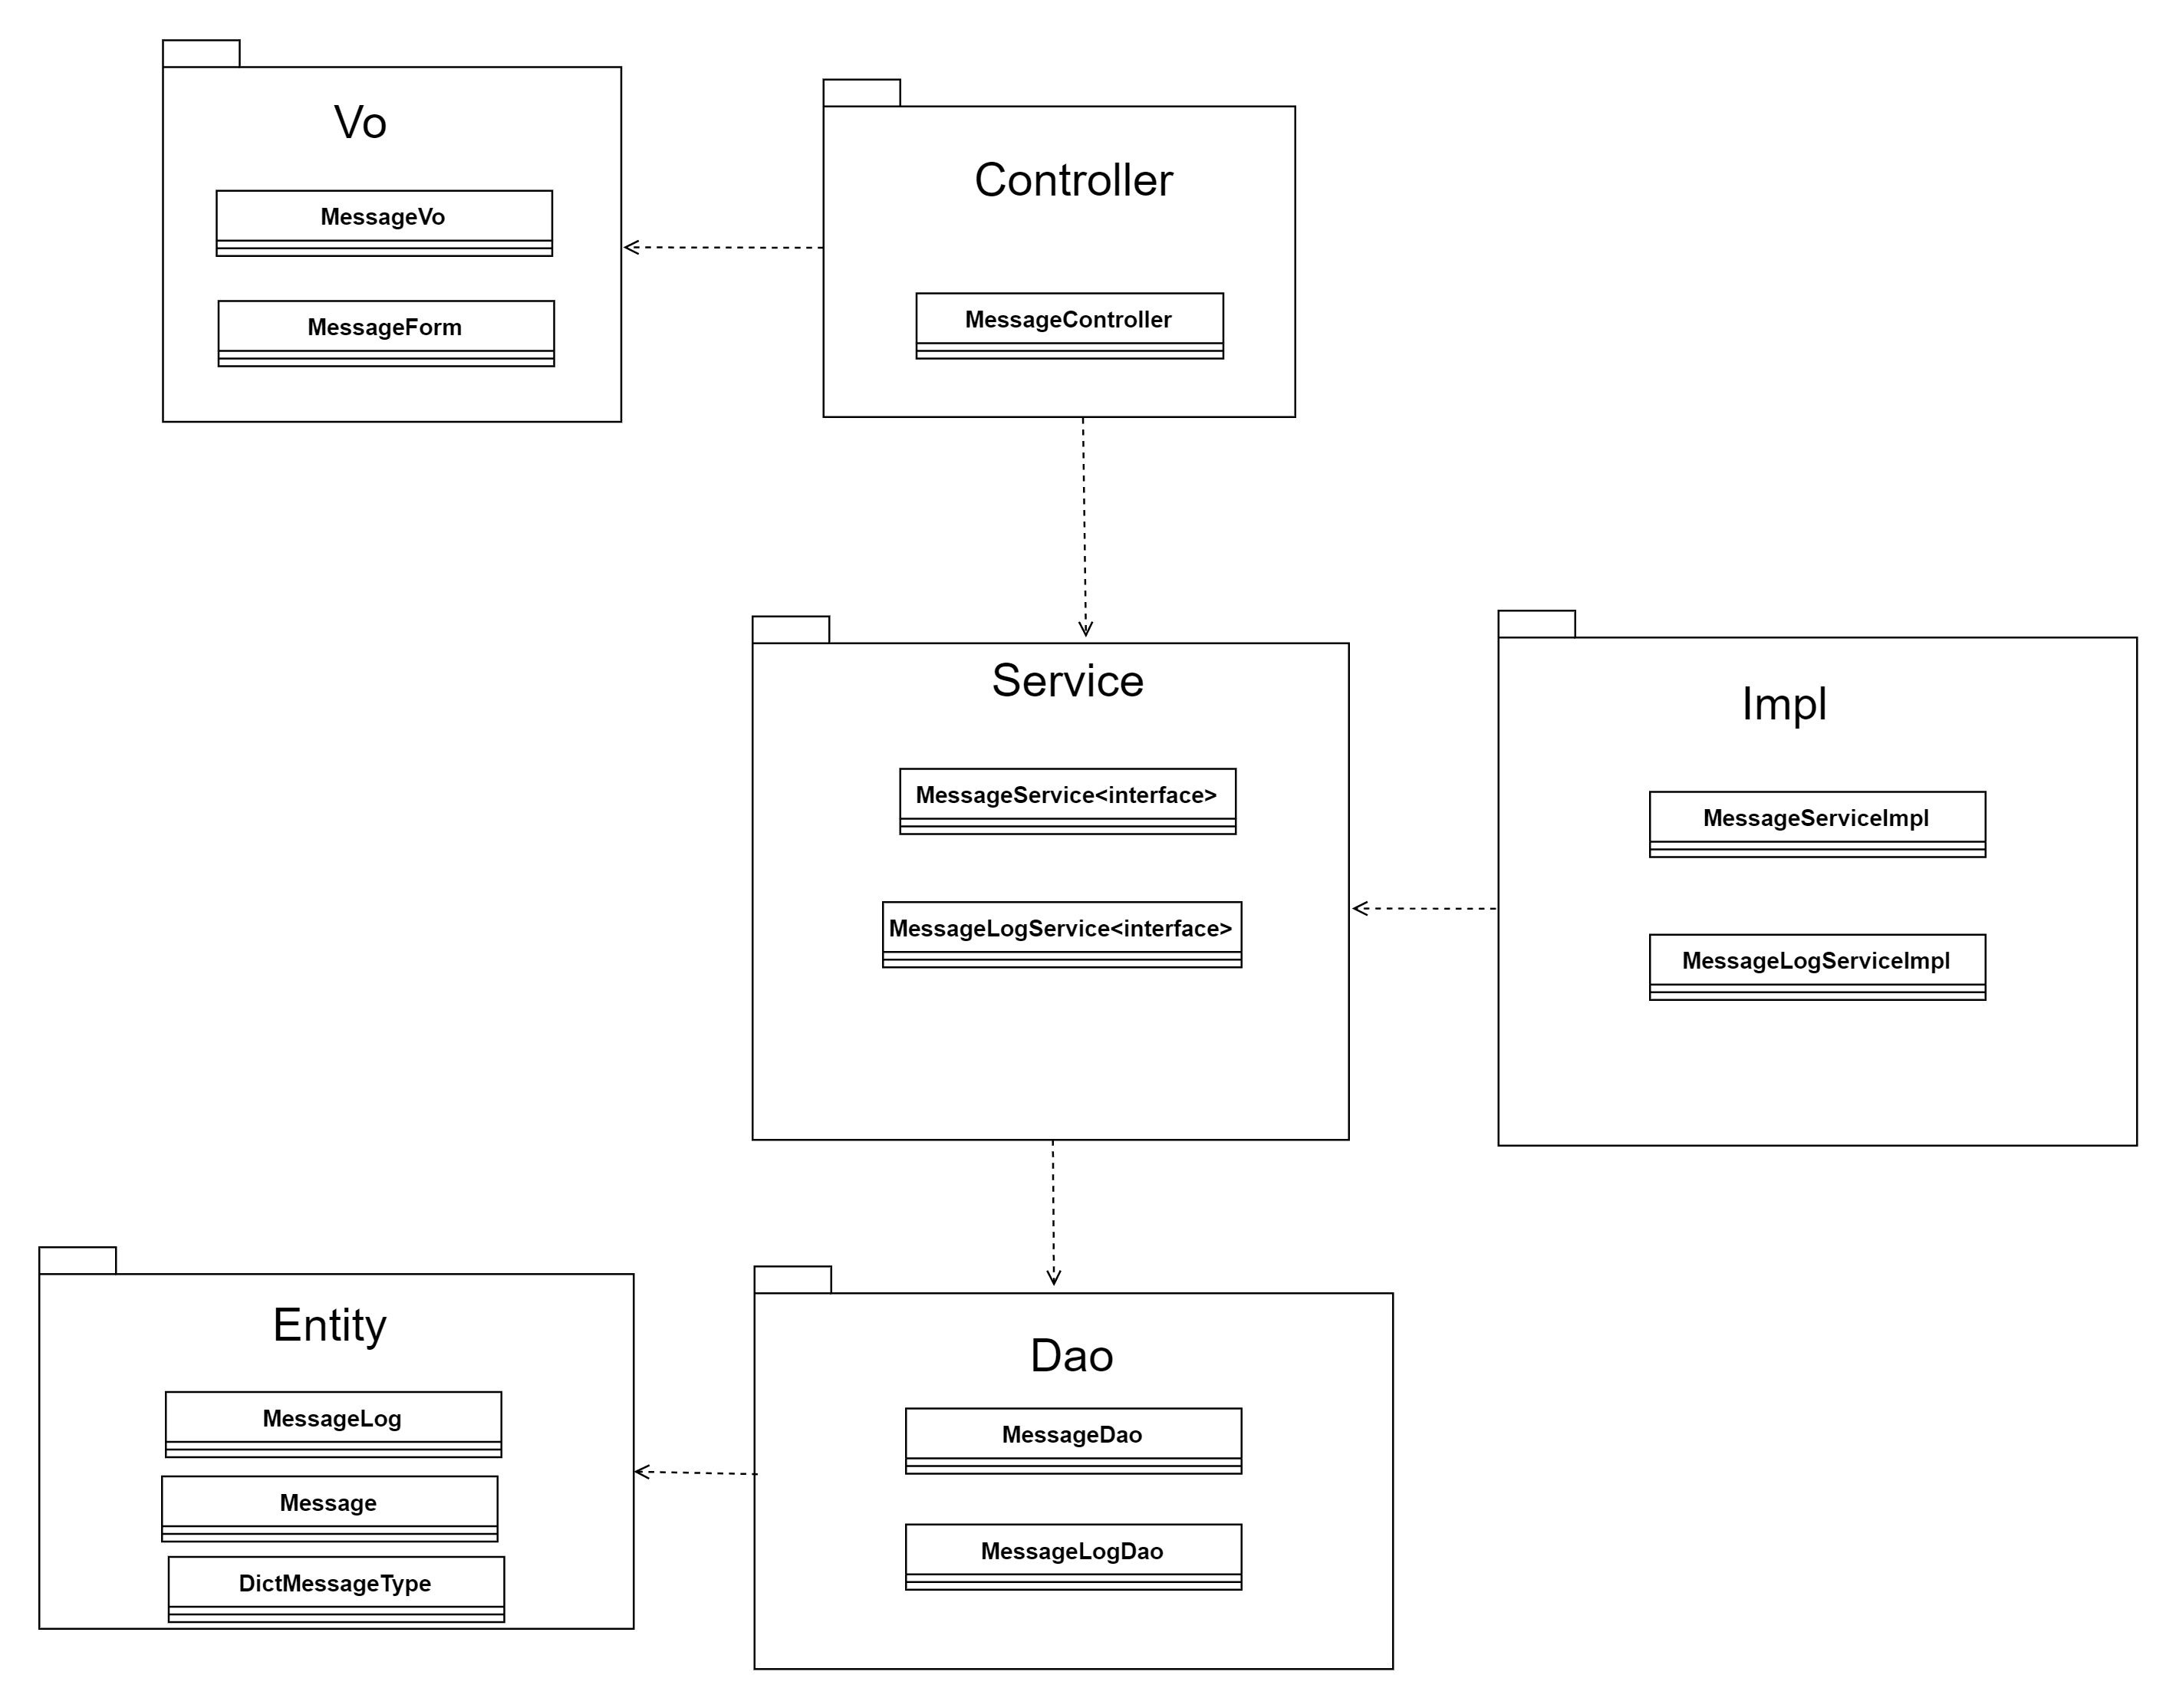
\includegraphics[width=\textwidth]{ch3/MessageService.jpg}
    \caption{MessageService模块包图}\label{fig:MessageService}
    \vspace{\baselineskip} % 表示图与正文空一行
\end{figure}


\subsection{GateWay网关模块}
GateWay网关模块负责路由转发,同时还负责初步的用户权限检查。所谓的网关权限检查,即对于用户的登陆凭证token进行初步检验。由于路由转发功能在配置文件中
已经实现,需要自定义的权限检查只需要一个包即可。下面为GateWay网关模块的包图~\ref{fig:GateWay}~。
\begin{figure}[htbp]
    \centering
    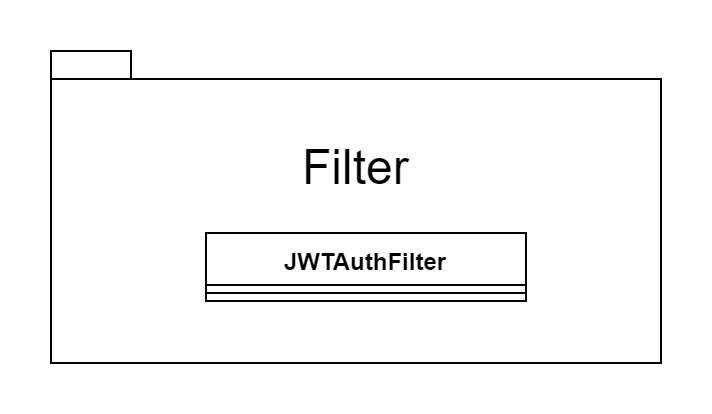
\includegraphics[width=0.7\textwidth]{ch3/GateWay.jpg}
    \caption{GateWay模块包图}\label{fig:GateWay}
    \vspace{\baselineskip} % 表示图与正文空一行
\end{figure}

\subsection{系统部署图}
本系统的部署主要涉及到服务端、客户端和数据库。客户端主要为Web浏览器,服务端需要部署多个微服务,同时启动Redis服务,数据库使用MySQL数据库。
系统部署图如图~\ref{fig:goujian}~所示。
\begin{figure}[htbp]
    \centering
    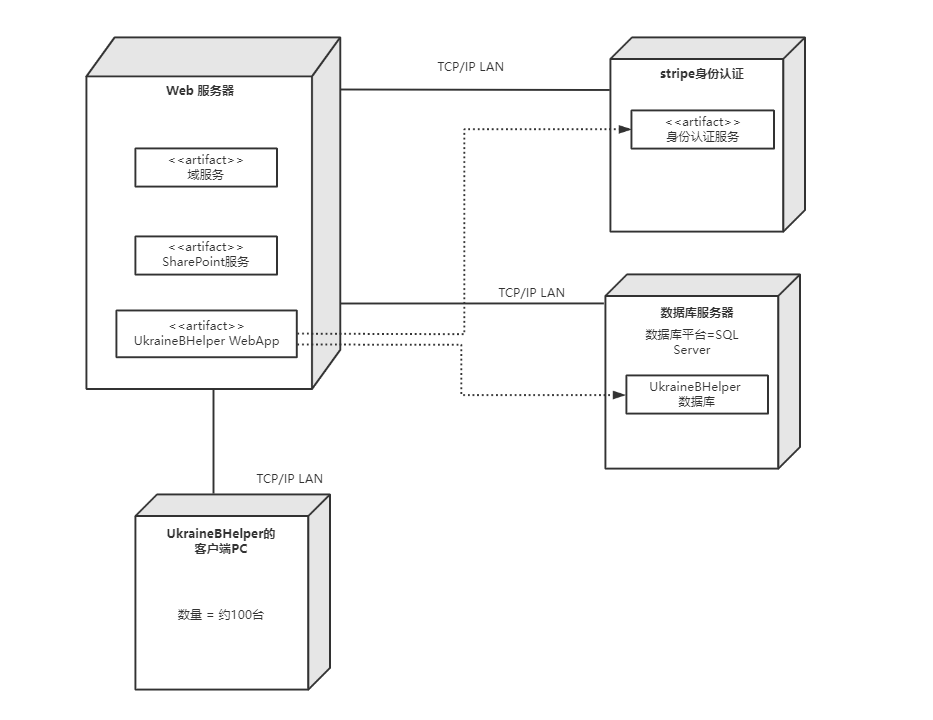
\includegraphics[width=\textwidth]{ch3/goujian.png}
    \caption{系统部署图}\label{fig:goujian}
    \vspace{\baselineskip} % 表示图与正文空一行
\end{figure}